\documentclass[11pt, oneside]{article}
\usepackage{geometry}
\geometry{letterpaper}
\usepackage{graphicx}
\usepackage{amssymb}
\usepackage[affil-it]{authblk}
\usepackage{verbatim}

\title{CompGO vignette}
\author{Sam Bassett, Ash Waardenberg}
\affil{Developmental and Stem Cell Biology Lab,\\Victor Chang Cardiac Research Institute,\\Darlinghurst, Sydney, Australia}
\date{}

\usepackage{Sweave}
\begin{document}
\maketitle
%\VignetteIndexEntry{Introduction}
\section{Introduction}
This package contains functions to accomplish several tasks relating to gene ontology enrichment comparison and visualisation given either .bed files or gene lists. It interfaces with rtracklayer and VariantAnnotation to easily annotate .bed files with genes, and with RDAVIDWebService to generate functional annotation charts based on these gene lists. From here, we provide several methods for comparative visualisation, including viewing the GO term hierarchy in two samples using a directed acyclic graph (DAG), performing z-score standardisation (approximately normal using a log odds-ratio (OR) - Equation 1 and 2) of GO terms returned from DAVID and comparing enrichment via pairwise scatterplots with linear fit and Jaccard metrics (Equation 3). We also provide functions to enable large-scale clustering.\\

\begin{equation}
Z \sim N(log(OR), \sigma^{2})
\end{equation}

\begin{equation}
z_{i} = \frac{log(OR)}{SE(OR)}
\end{equation}

\begin{equation}
J_{c} = \frac{A \cap B }{A \cup B}
\end{equation}


\section{Annotating .bed files}

The first step in this analysis pipeline is to generate individual Gene Ontology data for each dataset. We provide an interface to generate a list of genes from input .bed coordinates with the function anotateBedFromDb, which can take either a system path or a GRanges object as input:
\begin{Schunk}
\begin{Sinput}
> library(CompGO)
> library(TxDb.Mmusculus.UCSC.mm9.knownGene)
> data(bed.sample)
> # Here we create the GRanges object:
> sample.range = GRanges(seqnames=bed.sample$chr,
+     IRanges(start=bed.sample$start, end=bed.sample$end))
> # Note that the window around the .bed region beyond which
> # genes are cutoff is 5kb, this is modifiable
> sample.annotated = annotateBedFromDb(gRanges = sample.range,
+     db = TxDb.Mmusculus.UCSC.mm9.knownGene)
> head(sample.annotated)
\end{Sinput}
\begin{Soutput}
GRanges with 6 ranges and 2 metadata columns:
      seqnames               ranges strand |     tx_id         gene_id
         <Rle>            <IRanges>  <Rle> | <integer> <CharacterList>
  [1]     chr1 [74331608, 74400266]      + |       476           56695
  [2]     chr1 [74331608, 74400266]      + |       477           56695
  [3]     chr1 [74334821, 74350910]      - |      1990           69660
  [4]     chr1 [79790896, 79855240]      - |      2065           20720
  [5]     chr1 [79811683, 79855240]      - |      2066           20720
  [6]    chr10 [66558873, 66689664]      + |     30926          108829
  ---
  seqlengths:
           chr1         chr2         chr3 ...  chrY_random chrUn_random
      197195432    181748087    159599783 ...     58682461      5900358
\end{Soutput}
\end{Schunk}

\section{Generation of Gene Ontology data}
Once we have this annotated GRanges object, we can derive a list of genes to query DAVID and retrieve a full functional annotation chart. Alternatively, a list of genes can be directly supplied to DAVID. Note that there are several parameters available for tweaking the results returned from DAVID. Users can specify PVal and count; however, by default, no thresholding is performed. Since DAVID requires registration before the use of their Web Service R package, you should register first then substitute the placeholder email for your own.
\begin{Schunk}
\begin{Sinput}
> # fnAnot = getFnAnot_genome(sample.annotated$gene_id,
> #    email = "P.Lace-holder@inst.edu", listName="sample")
> # We instead use examples taken from the RDAVIDWebService package
> # to illustrate the utility of this package:
> data(funChart1)
> data(funChart2)
> funChart1 = subset(funChart1, Category %in%
+     c("GOTERM_BP_ALL", "GOTERM_MF_ALL", "GOTERM_CC_ALL"))
> funChart2 = subset(funChart2, Category %in%
+     c("GOTERM_BP_ALL", "GOTERM_MF_ALL", "GOTERM_CC_ALL"))
> str(funChart1)
\end{Sinput}
\begin{Soutput}
'data.frame':	141 obs. of  13 variables:
 $ Category       : Factor w/ 4 levels "GOTERM_BP_ALL",..: 2 2 2 3 3 1 1 3 1 3 ...
 $ Term           : Factor w/ 149 levels "GO:0000267~cell fraction",..: 15 109 17 72 74 30 52 115 136 13 ...
 $ Count          : int  40 24 19 6 8 18 10 8 18 11 ...
 $ X.             : num  25.81 15.48 12.26 3.87 5.16 ...
 $ PValue         : num  2.45e-07 4.32e-06 1.59e-05 3.32e-05 8.60e-05 ...
 $ Genes          : Factor w/ 118 levels "1403_S_AT, 37898_R_AT, 1983_AT, 35373_AT, 1910_S_AT",..: 54 38 41 102 75 57 51 75 49 27 ...
 $ List.Total     : int  134 134 134 132 132 138 138 132 138 132 ...
 $ Pop.Hits       : int  2010 960 685 43 121 615 193 129 681 308 ...
 $ Pop.Total      : int  15908 15908 15908 15143 15143 14116 14116 15143 14116 15143 ...
 $ Fold.Enrichment: num  2.36 2.97 3.29 16.01 7.58 ...
 $ Bonferroni     : num  0.000056 0.000985 0.003622 0.013907 0.035652 ...
 $ Benjamini      : num  0.000056 0.000493 0.001209 0.013907 0.017988 ...
 $ FDR            : num  0.000314 0.005536 0.020375 0.046636 0.120851 ...
\end{Soutput}
\begin{Sinput}
> # once the charts have been retrieved, they can be written
> # to disk for subsequent batch processing like so:
> # write.table(funChart1, "./path/to/text.txt")
\end{Sinput}
\end{Schunk}

\section{Analysis and comparison}

If you have multiple functional annotation charts, you can start directly comparing and visualising them in a pairwise manner. If you had output many functional annotation charts to a directory, it's possible to generate a matrix using the zTransformDirectory function. This table can then be used as an input to clustering functions (under development). Below, we will consider two ways of visualising the differences between sets using pairwise scatterplots (Figure 1) and a directed acyclic graph (Figure 2).\\
Figure 1: Pairwise scatterplot. The level of gene overlap between two sets is shown as the Jaccard coefficient, and the overall similarity between the GO enrichments is represented by the correlation. Using these examples, it can be noted that there is little gene overlap as well as little correlation.\\
\begin{figure}
\begin{center}
\begin{Schunk}
\begin{Sinput}
> plotZScores(funChart1, funChart2)
\end{Sinput}
\begin{Soutput}
[1] "0.0068"
\end{Soutput}
\end{Schunk}
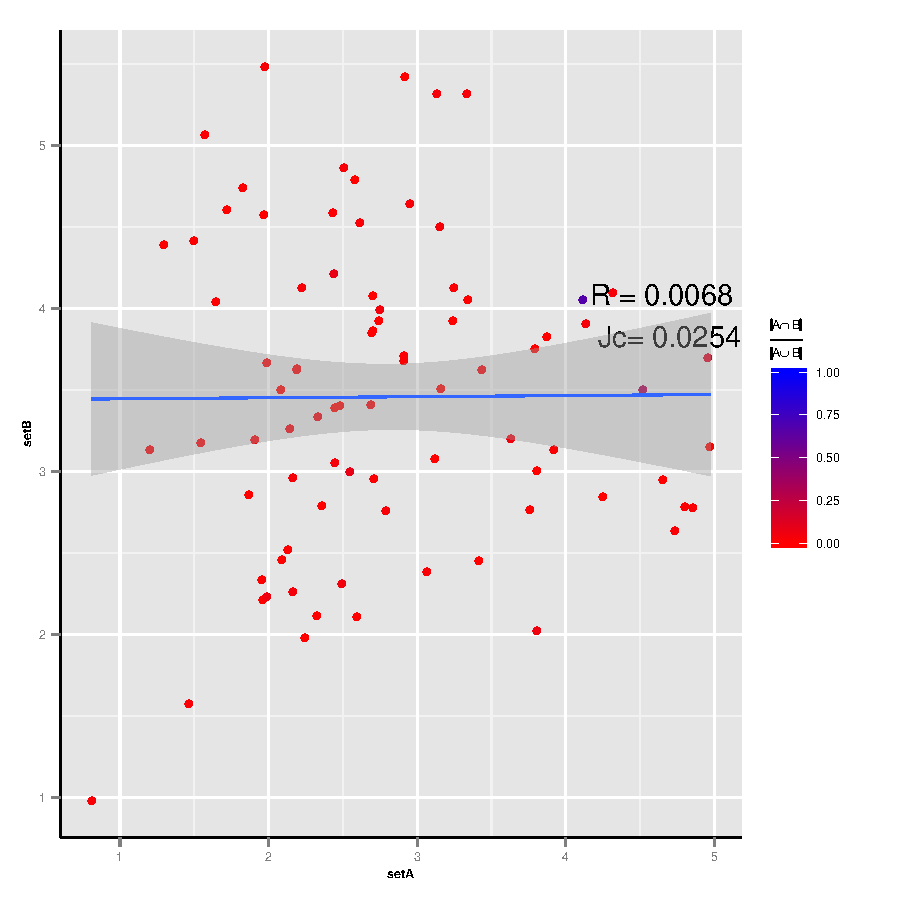
\includegraphics{CompGO-fig1}
\end{center}
\caption{Pairwise plot of Z scores for the two datasets. Gene ontology terms are coloured by their Jaccard coefficient as represented in the legend.}
\label{fig:one}
\end{figure}

Figure 2: Directed Acyclic Graph (DAG). In addition to pairwise plots, which provide an overview of the comparison, a great way to visualise the differences between two sets is to use a DAG of GO terms. Here, we colour each node based on the set or combinations of sets it originated from - yellow nodes are shared between two, red ones are the first input set, green ones are the second. In this case, there are several clear differences - funChart1 is enriched in oxygen and haeme binding, while funChart2 contains terms for transferase and protein kinase activity (Figure 2).\\
\begin{figure}
\begin{center}
\begin{Schunk}
\begin{Sinput}
> plotTwoGODags(funChart1, funChart2, ont="MF", cutoff=0.01)
\end{Sinput}
\end{Schunk}
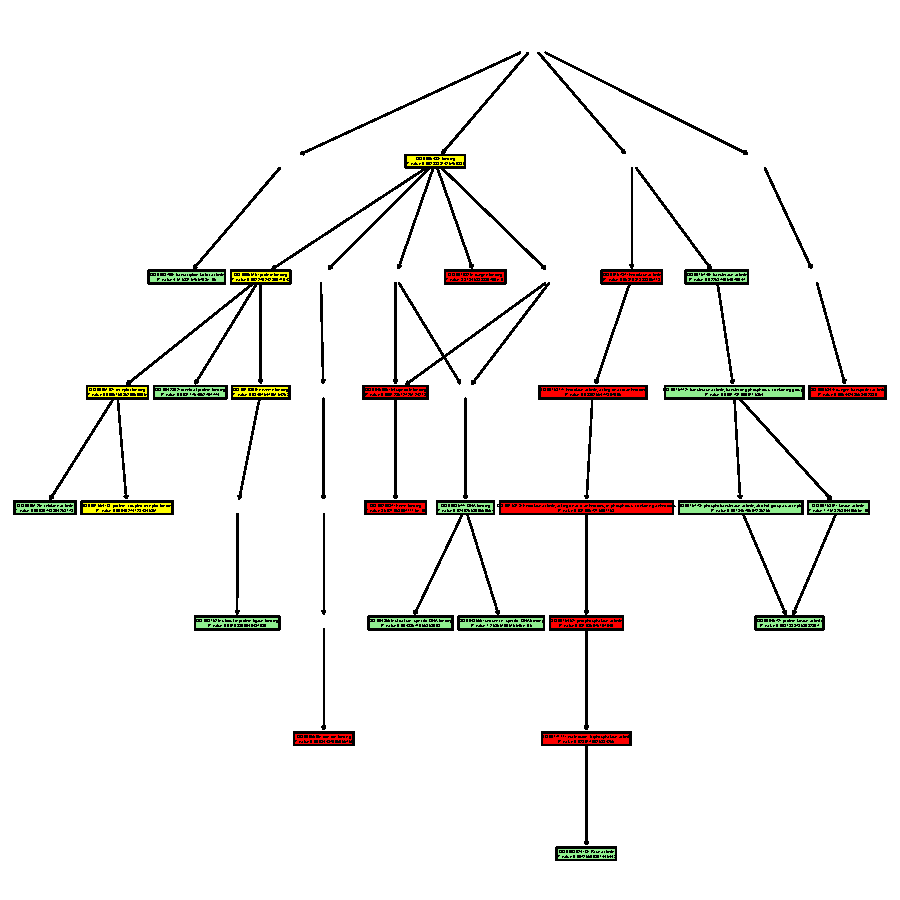
\includegraphics{CompGO-fig2}
\end{center}
\caption{Directed acyclic graph showing differences in GO term enrichment: yellow means the term is present in both sets, red means the first input set, green means the second.}
\label{fig:two}
\end{figure}

\end{document}
